%-----------Procedimiento  

\section*{Procedimiento}

\noindent Para poder comenzar con esta pr\'actica selecione cuatro trazas al azar de los sets proporcionados,
 dichas trazas son:

\begin{description}
    \item[SetA] - hop02
    \item[SetD] - hop04
    \item[SetG] - hop21
    \item[SetF] - hop29 
\end{description}

\noindent El siguiente paso es crear un script en AWK para generar las trazas del proceso RTT (\emph{sampleRTT}),
su estimaci\'on (\emph{estimatedRTT}) y el valor del temporizador (\emph{TimeoutInterval}). La base para este script 
son las secciones 2.1 a 2.3 del \textbf{RFC 6298}. En la figura siguiente se puede ver el c\'odigo del script

\begin{figure}[H]
    \centering
    \begin{lstlisting}[frame=single, breaklines=true, basicstyle=\footnotesize\ttfamily, breakatwhitespace=false, 
        columns=flexible, tabsize=2, showstringspaces=false, language=AWK] 
        BEGIN {
            # Inicializacion de parametros
            alpha = 1/8    # Suavizado para SRTT
            beta = 1/4     # Suavizado para RTTVAR
            K = 4          # Factor para RTTVAR
            RTO = 1        # Valor inicial de RTO
            firstRTT = 1   # Bandera para la primera medicion RTT
            sample_count = 0  # Contador de muestras procesadas
            start_sample = 200  # Comenzar a partir de la muestra 200
            max_samples = 30     # Tomar solo 30 muestras
        }
        
        {
            # Incrementar el contador de muestras
            sample_count++
        
            # Solo procesar muestras a partir de la muestra 200
            if (sample_count >= start_sample && sample_count < start_sample + max_samples) {
                # RTT_value es el unico valor por linea
                RTT = $1
        
                # Primer RTT
                if (firstRTT == 1) {
                    SRTT = RTT
                    RTTVAR = RTT / 2
                    RTO = SRTT + K * RTTVAR
                    firstRTT = 0
                } else {
                    # RTT subsecuentes
                    RTTVAR = (1 - beta) * RTTVAR + beta * (SRTT > RTT ? SRTT - RTT : RTT - SRTT)
                    SRTT = (1 - alpha) * SRTT + alpha * RTT
                    RTO = SRTT + K * RTTVAR
                }
        
                # Escribir en los archivos de salida
                print RTT >> "sampleRTT"
                print SRTT >> "estimatedRTT"
                print RTO >> "timeoutInterval"
            }
        
            # Si ya se procesaron 30 muestras, terminamos el script
            if (sample_count >= start_sample + max_samples) {
                exit
            }
        }
        
        END {
            print "Proceso completado. Los archivos de salida son: sampleRTT, EstimatedRTT, TimeoutInterval."
        }
        
    \end{lstlisting}
    \caption{Script para extraer los datos requeridos}
    \label{fig:scriptAWK}
\end{figure}

\noindent Una vez creado lo ejecutamos para cada una de las trazas seleccionadas, a continuaci\'on se muestra la forma de
ejecuci\'on 

\begin{figure}[H]
    \centering
    \begin{lstlisting}[frame=single, breaklines=true, basicstyle=\footnotesize\ttfamily, breakatwhitespace=false, 
        columns=flexible, tabsize=2, showstringspaces=fals] 
        awk -f rfc6298.awk hop02.txt
    \end{lstlisting}
    \caption{Ejecuci\'on del script para la traza \textit{hop02.txt}}
    \label{fig:execScript}
\end{figure}

\noindent Como se puede ver en la \textit{Figura \ref*{fig:scriptAWK}} al ejecutar el script se generan tres trazas: 
\textbf{sampleRTT}, \textbf{estimatedRTT} y \textbf{timeoutInterval}. El siguiente paso es crear las instrucciones en 
\textit{Octave} para poder visualizar en una sola gr\'afica: la traza original y las trazas generadas por el script. 
A continuaci\'on se muestran las instrucciones propuestas, a reserva del nombre de los ejes y el titulo que cambiar\'a
al graficar cada una de las trazas. Adem\'as veremos las gr\'aficas creadas por defecto.

\begin{figure}[H]
    \centering
    \begin{lstlisting}[frame=single, breaklines=true, basicstyle=\footnotesize\ttfamily, breakatwhitespace=false, 
        columns=flexible, tabsize=2, showstringspaces=fals] 
        load estimatedRTT;
        load timeoutInterval;
        plot(sampleRTT, '--*', 'Color', 'b', 'LineWidth', 0.5, 'MarkerSize', 8);
        hold on;
        plot(estimatedRTT, '--*', 'Color', 'k', 'LineWidth', 0.5, 'MarkerSize', 8);
        plot(timeoutInterval, '--*', 'Color', 'r', 'LineWidth', 0.5, 'MarkerSize', 8);
        legend('sampleRTT','estimatedRTT','timeoutInterval');
        grid on;
        xlabel('Eje x');
        ylabel('Eje y');
        title('Erro incurrido');
        print -dpng "traza.png";
    \end{lstlisting}
    \caption{Ejecuci\'on del script para la traza \textit{hop02.txt}}
    \label{fig:execScript}
\end{figure}

\newpage

\begin{figure}[H]
	\centering
	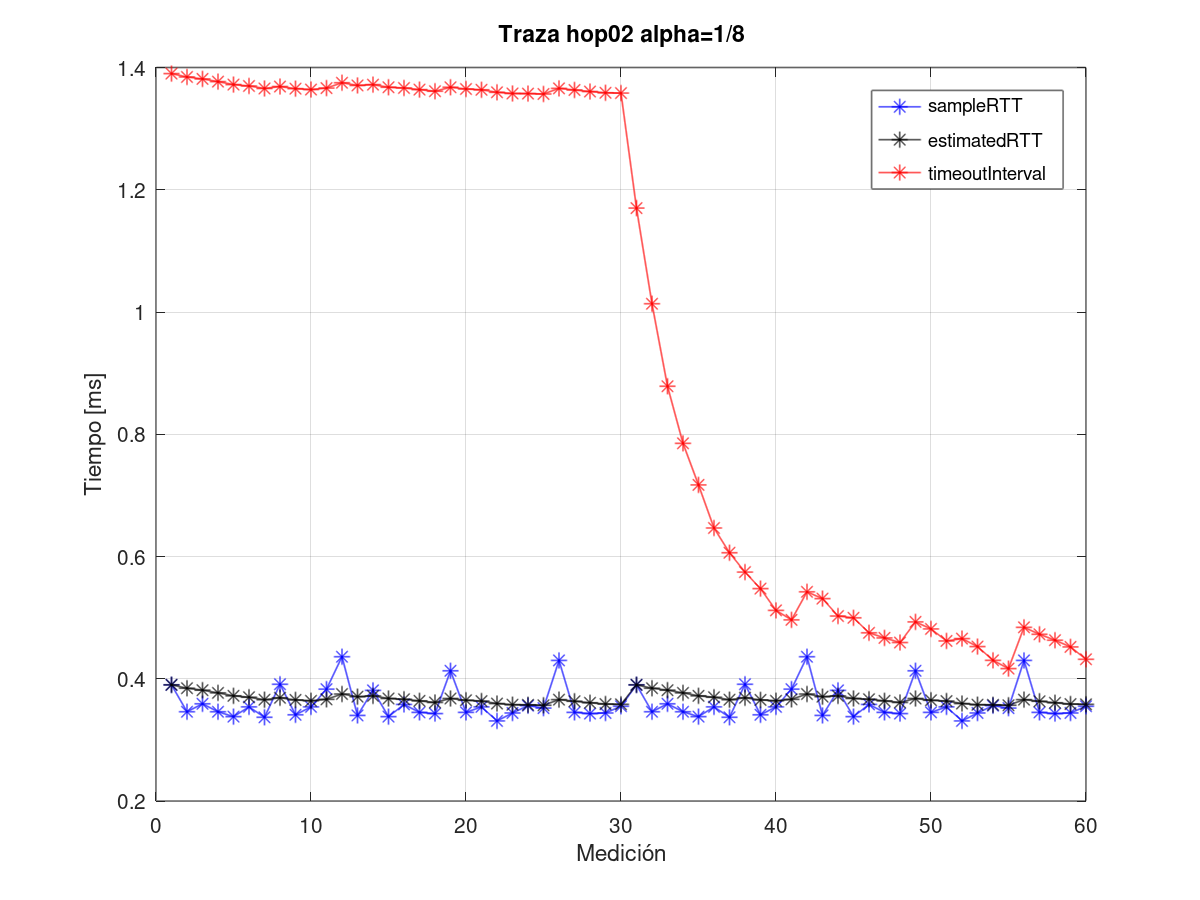
\includegraphics[width=0.8\textwidth]{img/alpha18/trazahop02.png}
	\caption{Gr\'afica de las trazas de las muetras hop02}
    
	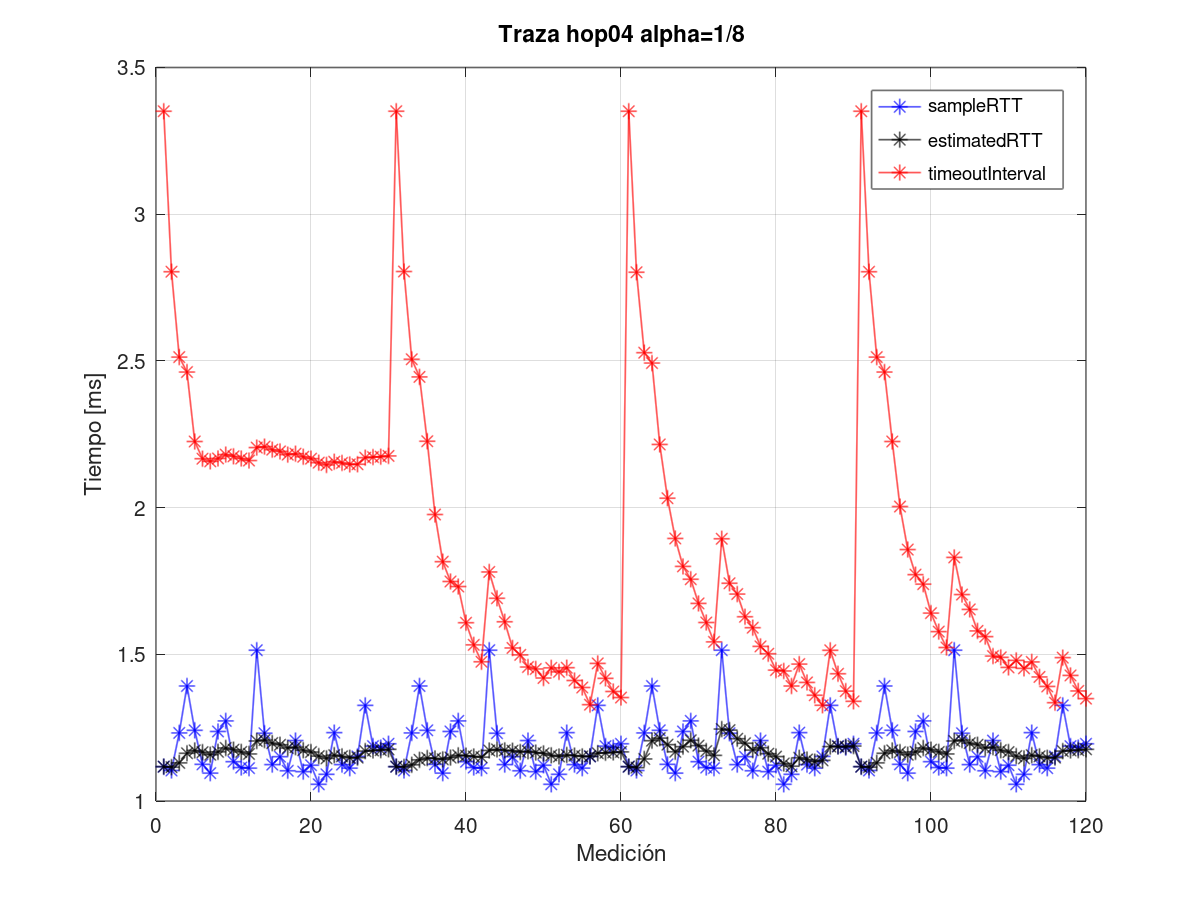
\includegraphics[width=0.8\textwidth]{img/alpha18/trazaHop04.png}
	\caption{Gr\'afica de las trazas de las muetras hop04}
\end{figure}

\begin{figure}[H]
	\centering
	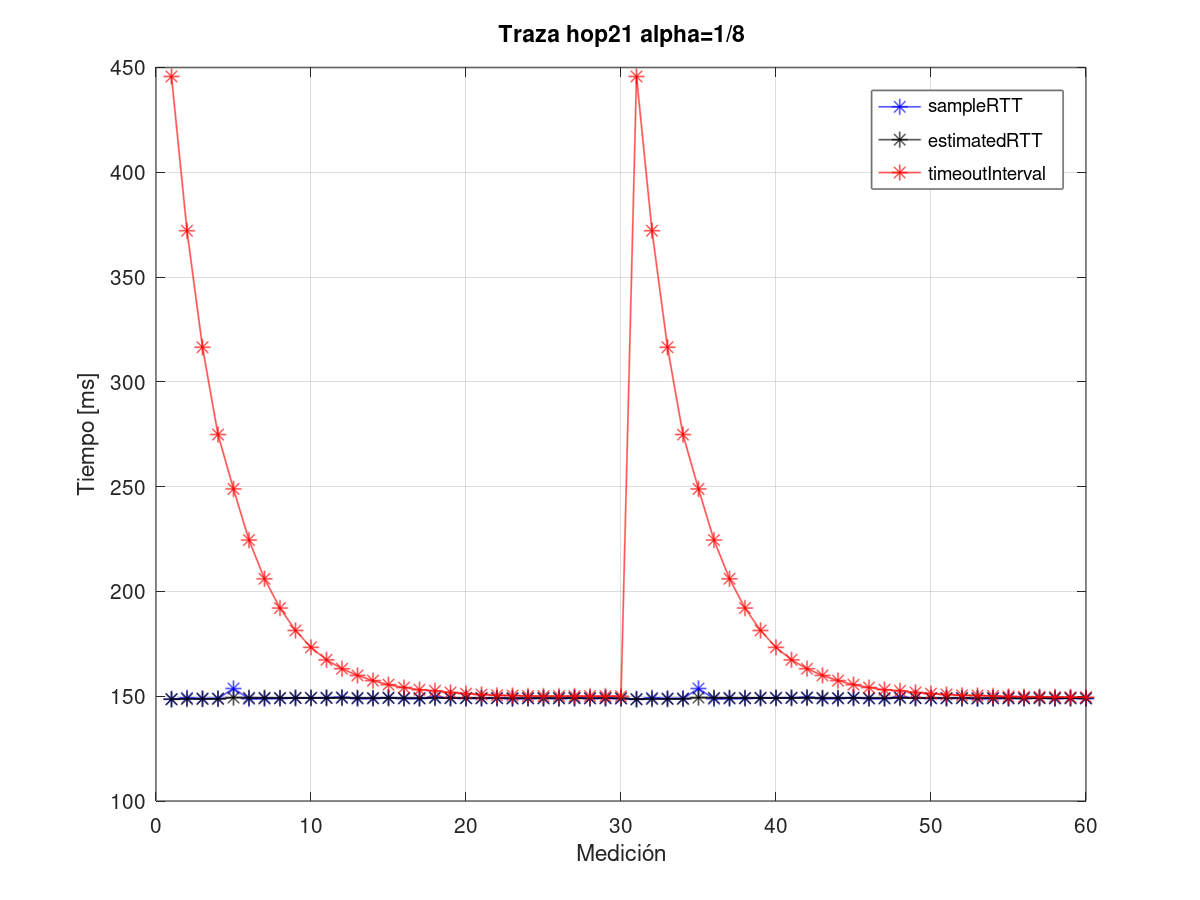
\includegraphics[width=0.8\textwidth]{img/alpha18/trazaHop21.png}
	\caption{Gr\'afica de las trazas de las muetras hop21}
	\label{fig:hop21Graph}
\end{figure}

\begin{figure}[H]
	\centering
	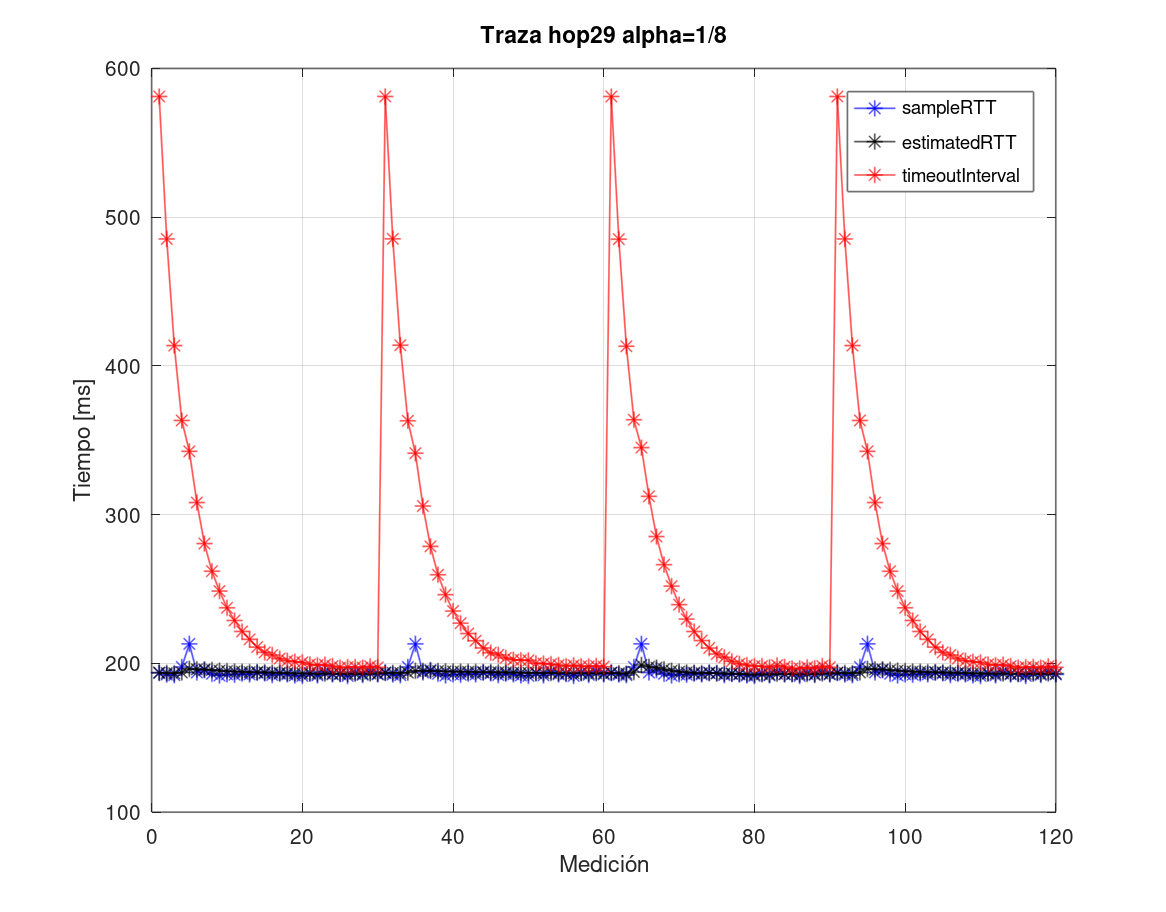
\includegraphics[width=0.8\textwidth]{img/alpha18/trazaHop29.png}
	\caption{Gr\'afica de las trazas de las muetras hop29}
	\label{fig:hop29Graph}
\end{figure}

\newpage
\subsection*{Cuestionario}

\begin{enumerate}
    \item ¿Se observa un proceso suave en el proceso de estimaci\'on (\textit{EstimatedRTT}) con
    respecto a las muestras del RTT (\textit{SampleRTT}) tal como propone Jacobson?
    \item[] Si, el proceso de estimaci\'on de \textit{EstimatedRTT} deber\'ia ser suave con respectoa
    a las muestras de \textit{SampleRTT}, como lo propone el algoritmo de Jacobson
    
    \item Las f\'ormulas de Van Jacobson para el c\'alculo del RTO son las siguientes:
    $$EstimatedRTT = (1-\alpha) * EstimatedRTT + \alpha * R^\prime$$
    $$VariacionRTT = (1-\beta) * VariacionRTT + \beta * |EstimatedRTT-R^\prime|$$
    $$TimeoutInterval = EstimatedRTT + max(G, K*VariacionRTT)$$
    \item[] Los valores por defecto son \(\alpha=1/8\) y \(\beta=1/4\) son ampliamente utilizados
    en la pr\'actica debido a que equilibran adecuadamente la estabilidad de la estimaci\'on de RTT
    y la sensibilidad a las fluctuaciones de la red.
    \item[] \(\alpha\) controla que tan r\'apido se adapra el \textit{EstimatedRTT} a nuevos valores
    de \textit{SampleRTT}. Si el RTT flut\'ua constantemente debido a cambios r\'apidos en la red, es
    posible que se quiera una estimaci\'on m\'as precisa con menor error. \(\alpha\) podr\'ia ser
    ajustado ligeramente a un valor m\'as bajo, por ejemplo, \(\alpha=1/16\) para hacer la estimaci\'on
    m\'as conservadora y menos sensible a fluctuaciones grandes, pero esto har\'a que el \textit{EstimatedRTT}
    sea menos reactivo.
\end{enumerate}